\documentclass[tikz,border=5mm]{standalone}
\usepackage[utf8]{inputenc}
\usepackage[T1]{fontenc}
\usepackage{lmodern}
\renewcommand{\familydefault}{\sfdefault}

\usetikzlibrary{positioning, arrows.meta, shapes.geometric, fit, backgrounds, calc}

% --- "Slate and Stone" palette ---
\definecolor{polysakColor}{RGB}{120,130,140}
\definecolor{fettColor}{RGB}{110,95,80}
\definecolor{proteinColor}{RGB}{58,78,100}
\definecolor{sukkerColor}{RGB}{195,205,215}
\definecolor{lipidLight}{RGB}{225,215,200}
\definecolor{aminoColor}{RGB}{150,165,185}
\definecolor{glykbg}{RGB}{180,190,200}
\definecolor{pyroxbg}{RGB}{165,150,130}
\definecolor{krebsbg}{RGB}{215,205,190}
\definecolor{oksfosbg}{RGB}{70,85,105}
\definecolor{accentDark}{RGB}{40,50,65}
\definecolor{arrowGray}{RGB}{55,65,80}

% =====================================================
% Explicit coordinate grid 
% =====================================================
% Column x-coordinates
\def\colA{0}         % Primary macronutrients
\def\colB{4.2}       % Secondary metabolites
\def\colT{6.5}       % Aminosyrer trunk channel
\def\colRespWest{7.0}% EXACT LEFT EDGE for all respiration boxes
\def\colC{9.6}       % Center axis for respiration pathway (\colRespWest + 2.6cm)

\def\respWidth{5.2cm}% Standardized width for the entire respiration column

% Row y-coordinates (Expanded Glykolyse spacing)
\def\rowTop{0}      
\def\rowPyr{-2.2}    % Pushed down for more space
\def\rowPyrox{-3.9}  
\def\rowAcet{-5.6}   
\def\rowKrebs{-8.0}  
\def\rowOks{-11.0}   

% Calculated secondary rows
\def\rowGly{-1.1}       
\def\rowFett{-3.35}     
\def\rowTrunkTop{-2.45} % Locked exactly to \rowPyr - 0.25cm to force parallel straight line

\begin{document}
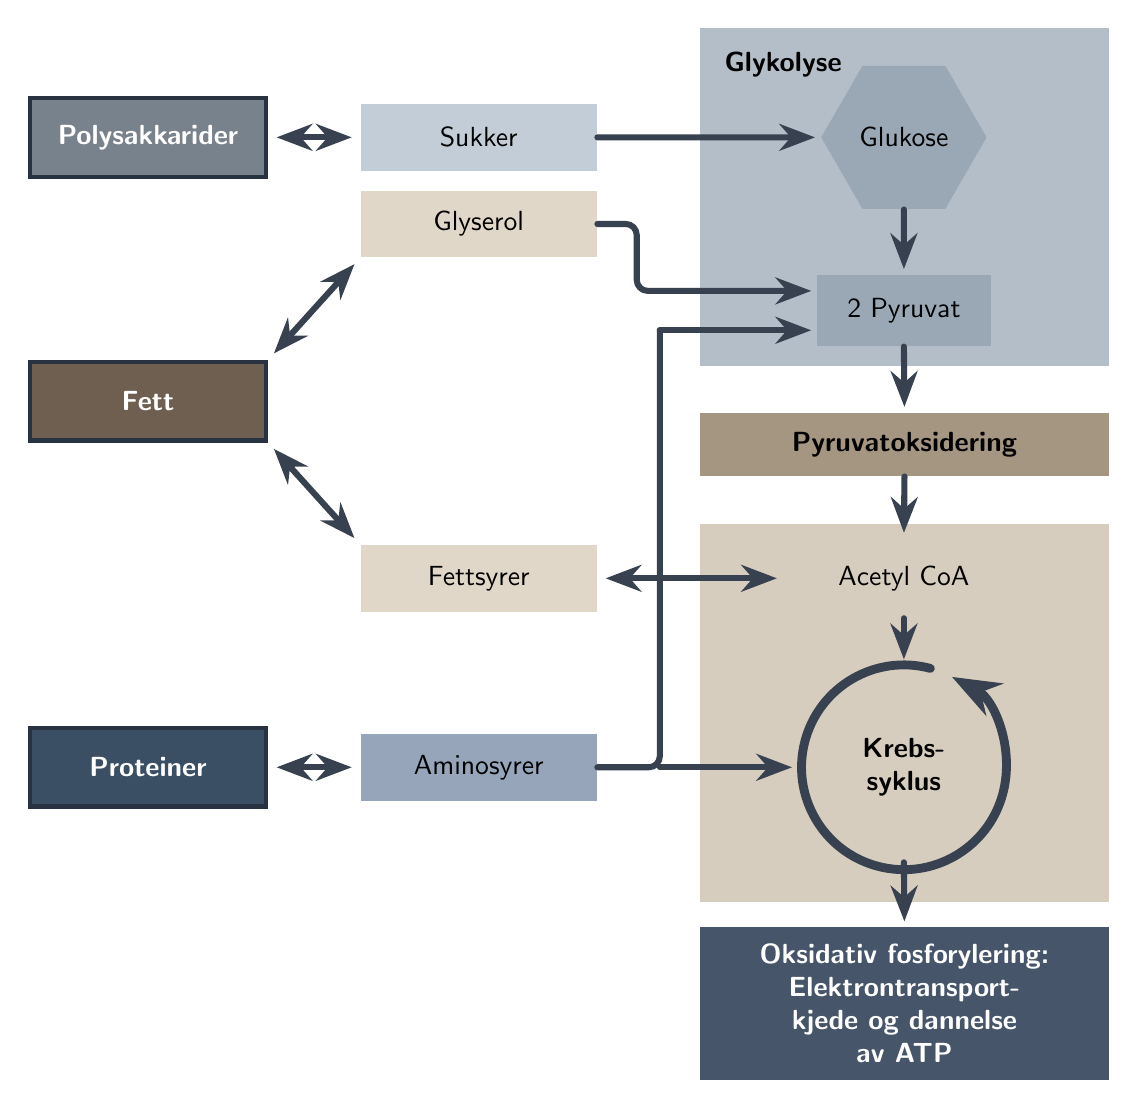
\begin{tikzpicture}[
    >={Stealth[scale=1.0]}, 
    arrow/.style       ={->,  line width=2.2pt, arrowGray, rounded corners=4pt, line cap=round, line join=round, shorten >=2pt},
    biarrow/.style     ={<->, line width=2.2pt, arrowGray, rounded corners=4pt, line cap=round, line join=round, shorten >=3pt, shorten <=3pt},
    trunk/.style       ={line width=2.2pt, arrowGray, rounded corners=4pt, line cap=round, line join=round},
    macroPrimary/.style={rectangle, draw=accentDark, line width=1.6pt,
                         minimum width=3.0cm, minimum height=1cm,
                         align=center, anchor=center, font=\bfseries, text=white},
    macroLight/.style  ={rectangle, draw=none, minimum width=3.0cm, minimum height=0.85cm,
                         align=center, anchor=center},
    respLabel/.style   ={rectangle, draw=none, align=center, anchor=center, minimum height=0.8cm, inner ysep=6pt},
    acetylBox/.style   ={rectangle, draw=none, minimum width=3.0cm, minimum height=1.0cm, align=center, anchor=center, inner ysep=6pt},
    glukoseStyle/.style={regular polygon, regular polygon sides=6, draw=none,
                         fill=glykbg!135, minimum width=2.1cm, inner sep=2pt, anchor=center},
    pyruvatStyle/.style={rectangle, draw=none, fill=glykbg!135,
                         minimum width=2.2cm, minimum height=0.9cm, align=center, anchor=center},
]

% =====================================================
% RIGHT COLUMN: respiration pathway
% =====================================================
\node[glukoseStyle]  (glukose) at (\colC,\rowTop)   {Glukose};
\node[pyruvatStyle]  (pyruvat) at (\colC,\rowPyr)   {2 Pyruvat};

% Strictly left-aligned flush boxes
\node[respLabel, fill=pyroxbg, minimum width=\respWidth, font=\bfseries, anchor=west] 
                     (pyrox)   at (\colRespWest, \rowPyrox) {Pyruvatoksidering};
                     
\node[respLabel, fill=oksfosbg, minimum width=\respWidth, minimum height=1.8cm, font=\bfseries, align=center, text=white, anchor=west]
                     (oksfos)  at (\colRespWest, \rowOks)
                     {Oksidativ fosforylering:\\Elektrontransport-\\kjede og dannelse\\av ATP};

\node[acetylBox]     (acetyl)  at (\colC,\rowAcet)  {Acetyl CoA};
\node[respLabel, minimum width=2.6cm, minimum height=2.4cm, font=\bfseries, align=center]
                     (krebs)   at (\colC,\rowKrebs) {Krebs-\\syklus};

% Glykolyse title placed top-left inside the background box
\node[font=\bfseries, anchor=north west] (glyktitle) at (\colRespWest+0.2, 1.2) {Glykolyse};

% Krebs cycle circular arrow 
\draw[line width=3.2pt, arrowGray, line cap=round, ->]
    (krebs.center) ++(75:1.3cm) arc[start angle=75, end angle=422, radius=1.3cm];

% Central vertical pathway arrows
\draw[arrow] (glukose.south) -- (pyruvat.north);
\draw[arrow] (pyruvat.south) -- (pyrox.north);
\draw[arrow] (pyrox.south)   -- (acetyl.north);
\draw[arrow] (acetyl.south)  -- ([yshift=1.3cm]krebs.center); 
\draw[arrow] (krebs.south)   -- (oksfos.north);

% =====================================================
% MIDDLE COLUMN: secondary metabolites
% =====================================================
\node[macroLight, fill=sukkerColor] (sukker)    at (\colB,\rowTop)   {Sukker};
\node[macroLight, fill=lipidLight]  (glyserol)  at (\colB,\rowGly)   {Glyserol};
\node[macroLight, fill=lipidLight]  (fettsyrer) at (\colB,\rowAcet)  {Fettsyrer};
\node[macroLight, fill=aminoColor]  (amino)     at (\colB,\rowKrebs) {Aminosyrer};

% =====================================================
% LEFT COLUMN: primary macronutrients
% =====================================================
\node[macroPrimary, fill=polysakColor] (polysak) at (\colA,\rowTop)   {Polysakkarider};
\node[macroPrimary, fill=fettColor]    (fett)    at (\colA,\rowFett)  {Fett};
\node[macroPrimary, fill=proteinColor] (prot)    at (\colA,\rowKrebs) {Proteiner};

% =====================================================
% Connecting arrows
% =====================================================
% Bidirectional 
\draw[biarrow] (polysak) -- (sukker);
\draw[biarrow] (prot)    -- (amino);
\draw[biarrow] (fett.north east) -- (glyserol.south west);
\draw[biarrow] (fett.south east) -- (fettsyrer.north west);

% Sukker -> Glukose
\draw[arrow] (sukker.east) -- (glukose.west);

% Glyserol -> Glycolysis 
\draw[arrow] (glyserol.east) -- ++(0.5,0) |- ([yshift=0.25cm]pyruvat.west);

% Fettsyrer <-> Acetyl CoA 
\draw[biarrow] (fettsyrer.east) -- (acetyl.west);

% =====================================================
% Aminosyrer trunk + branches 
% =====================================================
\draw[trunk] (amino.east) -- (\colT,\rowKrebs) -- (\colT,\rowTrunkTop);

% Branch 1 -> Krebs-syklus 
\draw[arrow] (\colT,\rowKrebs) -- (\colC-1.35,\rowKrebs);

% Branch 2 -> Glycolysis (Perfectly parallel due to \rowTrunkTop math)
\draw[arrow] (\colT,\rowTrunkTop) -- ([yshift=-0.25cm]pyruvat.west);

% =====================================================
% Background colored regions 
% =====================================================
\begin{scope}[on background layer]
    % Glykolyse Background (Height increased to 4.3cm)
    \node[fill=glykbg, minimum width=\respWidth, minimum height=4.3cm, anchor=north west]
          (glykbox) at (\colRespWest, 1.4) {};
          
    % Krebs-syklus Background 
    \node[fill=krebsbg, minimum width=\respWidth, minimum height=4.8cm, anchor=north west]
          (krebsbox) at (\colRespWest, -4.9) {};
\end{scope}

\end{tikzpicture}
\end{document}